\chapter{TINJAUAN PUSTAKA}
\label{chap:tinjauanpustaka}

% Ubah bagian-bagian berikut dengan isi dari tinjauan pustaka

\section{Hasil Penelitian Terdahulu}
\label{sec:hasilpenelitianterdahulu}

\subsection{Applying Generative Adversarial Networks to Intelligent Subsurface Imaging and Identification}
\label{sec:apllyingGANtoISII}

William Rice melakukan penelitian terkait penerapan metode GAN untuk mendeteksi objek bawah permukaan tanah. 
Dalam penelitiannya, objek yang dideteksi berupa silinder dengan 3 jenis bahan, yaitu besi, plastik, dan beton yang terkubur di bawah permukaan tanah. 
Penelitian ini menggunakan metode FDTD dalam modelnya. 
Hasil penelitian ini menunjukkan bahwa metode GAN dapat digunakan pada data GPR, baik dari data asli maupun data simulasi GPR. 
\emph{Class conditioning} dapat diterapkan pada metode GAN dalam menghasilkan \emph{training data} yang terlabel untuk klasifikasi.
Dengan \emph{training data} ini, terlihat bahwa augmentasi GAN dapat meningkatkan pengklasifikasi. \parencite{Rice2019ApplyingGA}.

\subsection{Early Detection of Near-Surface Void Defects in Concrete Pavement Using Drone Based Thermography and GPR Methods - Final Report}
\label{earlydetectionGPRmethod}

Zhigang Shen beserta tim melakukan penelitian dengan 2 metode berbeda dalam mendeteksi cavities pada beton yang masih baru dicetak, yaitu dengan pendekatan \emph{Infrared Thermographic} dan \emph{Ground Penetrating Radar} (GPR). 
Penelitian dengan pendekatan GPR bertujuan untuk mengetahui batasan penggunaan GPR pada beton pasca pengecoran. 
Untuk menghindari kerusakan pada beton pasca pengecoran, sebuah papan triplek digunakan sebagai penampang GPR agar tidak menyentuh beton secara langsung. 
Hasil penelitian menunjukkan bahwa GPR dapat menjadi metode \emph{non-destructive testing} (NDT) untuk mendeteksi \emph{cavities} dengan ukuran 3.8 cm hingga 10 cm pada saat 3 jam setelah pengecoran beton. \parencite{earlyDetectionofNearSurfaceVoidDefect}

\subsection{Image-to-Image Translation with Conditional Adversarial Networks}
\label{image2imagetranslationCGAN}
Philip Isola beserta timnya melakukan penelitian terkait penggunaan \emph{Conditional Adversial Networks} (cGAN) dalam mengubah dari suatu gambar ke gambar lain. 
Penelitian ini mendemonstrasikan penggunaan pix2pix dalam mensintesis foto dari bentuk label kasaran menjadi suatu gambar objek tertentu. 
Dari penelitian disimpulkan bahwa penggunaan cGAN sangat menjanjikan dalam permasalahan perubahan gambar satu ke gambar lain, terkhususnya yang membutuhkan output terstruktur. \parencite{image2imageCGAN}

\section{Cavities}
\label{sec:cavities}

\emph{Cavities} atau \emph{void}, merupakan suatu rongga kosong yang terbentuk pada beton akibat udara yang terperangkap di dalamnya. 
Ketika beton selesai dicor, sebagian besar udara yang terperangkap keluar dari campuran. 
Udara terperangkap yang tersisa dalam campuran kemudian menciptakan kekosongan udara pada beton. 
Cavities pada beton dapat ditimbulkan oleh berbagai sebab, diantaranya: Pemadatan yang dilakukan dengan vibrator kurang baik, 
karena jarak antar bekisting dengan tulangan atau jarak antar tulangan terlalu sempit sehingga bagian mortar tidak dapat mengisi rongga antara agregat kasar dengan baik. \parencite{analisakerusakanbeton}
Contoh bentuk cavities pada beton dapat dilihat pada gambar \ref{fig:voidOnConcrete}.

\begin{figure}[ht]
  \centering
  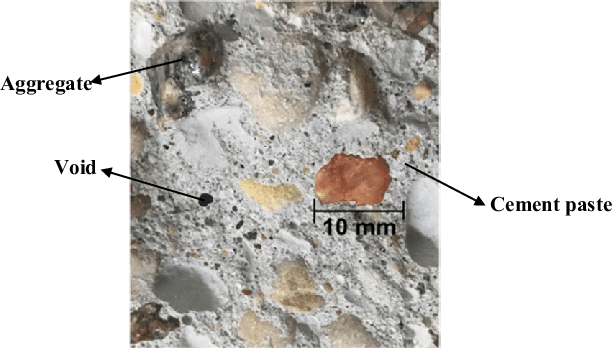
\includegraphics[scale=0.5]{gambar/voidOnConcrete.png}
  \caption{Bentuk Cavities pada Beton Kering \parencite{voidOnConcrete}.}
  \label{fig:voidOnConcrete}
\end{figure}

\section{Ground Penetrating Radar}
\label{sec:groundPenetratingRadar}

\emph{Ground Penetrating Radar} (GPR) merupakan salah satu metode geofisika dalam mengidentifikasi kondisi bawah permukaan. 
Penggunaan GPR pada awalnya digunakan untuk bahan geologi pada alam. 
Seiring berkembangnya teknologi, GPR dapat diterapkan untuk media jenis lainnya, seperti kayu, beton, dan aspal \parencite{jol2008ground}.

\begin{figure}[ht]
  \centering
  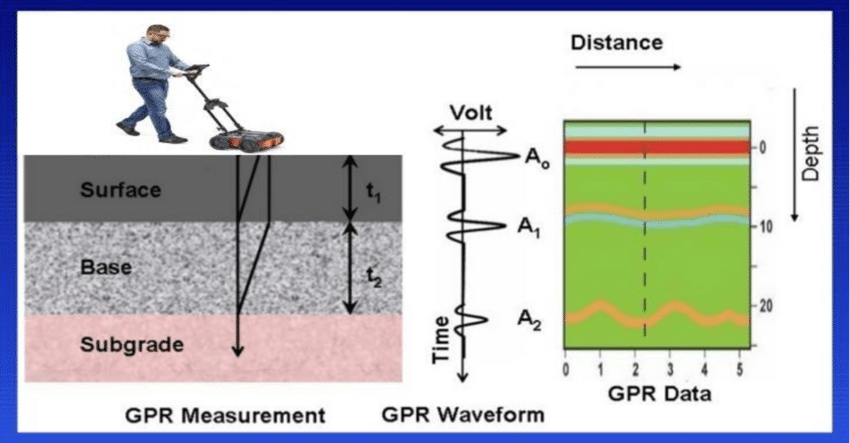
\includegraphics[scale=0.35]{gambar/prinsipGPR.png}
  \caption{Prinsip Kerja GPR Secara Umum \parencite{gprPrinciple}.}
  \label{fig:prinsipGpr}
\end{figure}

GPR terbagi menjadi 2 bagian, yaitu bagian antena pemancar (transmitter) dan bagian antena penerima (receiver). 
Garis besar sistem GPR dapat dilihat pada gambar \ref{fig:prinsipGpr}. 
Antena pemancar dan penerima biasanya identik dan memenuhi karakteristik bentuk gelombang yang dihasilkan. 
Antena pemancar membangkitkan sinyal listrik ke dalam tanah. 
Selama perambatan, sinyal akan mengalami berbagai kerugian (loss). 
Jika sinyal bertabrakan dengan bahan yang tidak homogen dengan media perambatan, maka sinyal akan dipantulkan. 
Sinyal ini akan diterima dan diproses oleh antena penerima.

Perambatan gelombang elektromagnetik diatur oleh sifat dielektrik medium yang dilaluinya, yaitu permitivitas dielektrik ($\varepsilon$), konduktivitas listrik ($\sigma$) dan permeabilitas magnetik ($\mu$). 
Secara khusus, permitivitas dielektrik dan konduktivitas listrik sangat mempengaruhi perilaku gelombang perambatan, masing-masing dalam hal kecepatan gelombang dan atenuasi gelombang, dan permeabilitas magnetik sama untuk semua bahan non-magnetik dengan permeabilitas magnetik ruang bebas $\mu_{0}$ dan tidak mempengaruhi perambatan dari gelombang EM. 
Kedalaman penetrasi dan resolusi spasial dipengaruhi oleh beberapa faktor, di antaranya adalah frekuensi sinyal yang dipancarkan dan jenis material yang diselidiki. \parencite{gprIntroduction}

Secara teoritis, nilai medan elektromagnetik dijelaskan melalui persamaan Maxwell : 

\begin{equation}
  \label{eq:maxWellE}
  \nabla  x \vec{E} = - \frac{ \delta  \vec{B}}{ \delta t} 
\end{equation}

\begin{equation}
  \label{eq:maxWellH}
  \nabla x  \vec{H}  =   \vec{J}  + \frac{ \delta  \vec{D} }{ \delta t} 
\end{equation}

\begin{equation}
  \label{eq:maxWellD}
  \nabla . \vec{D} =  q
\end{equation}

\begin{equation}
  \label{eq:maxWellB}
  \nabla . \vec{B} =  0
\end{equation}

Dimana $\vec{E}$ ($V.m^{-1}$) merupakan vektor kuat medan listrik, q ($C.m^{-3}$) merupakan kerapatan muatan listrik, $\vec{B}$ (T) merupakan vektor kerapatan fluks magnet, $\vec{J}$($A.m^{-2}$) merupakan vektor kerapatan arus listrik, $\vec{D}$ ($C.m^{-2}$) merupakan vektor perpindahan listrik, t (s) merupakan waktu, dan $\vec{H}$ ($A.m^{-1}$) merupakan vektor intensitas medan magnet. \parencite{jol2008ground}

Sebaliknya, perilaku medium tempat gelombang elektromagnetik merambat, dapat dijelaskan oleh hubungan konstitutif. 
Hubungan konstitutif adalah sarana untuk menggambarkan respons material terhadap bidang elektromagnetik. 
Secara matematis, hubungan konstitutif dirumuskan sebagai berikut:
\begin{equation}
  \label{eq:mediumJ}
  \vec{J} =  \sigma \vec{E}
\end{equation}

\begin{equation}
  \label{eq:mediumD}
  \vec{D} =  \varepsilon \vec{E}
\end{equation}

\begin{equation}
  \label{eq:mediumB}
  \vec{B} =  \mu \vec{H}
\end{equation}

Dengan menggabungkan teori medan EM dengan hubungan konstitutif, dimungkinkan untuk menggambarkan sinyal GPR secara komprehensif.


\subsection{GprMax}
\label{subsec:gprMax}

GprMax merupakan open source software yang mensimulasikan propagasi gelombang elektromagnetik. 
GprMax memecahkan persamaan Maxwell dalam 3D menggunakan metode Finite-Difference Time-Domain (FDTD). 
GprMax dirancang untuk pemodelan Ground Penetrating Radar (GPR) tetapi juga dapat digunakan untuk memodelkan propagasi gelombang elektromagnetik untuk banyak aplikasi lainnya. 

\begin{figure}[ht]
  \centering
  
\includegraphics[scale=0.35]{gambar/gprMax.png}
  \caption{Logo gprMax (sumber : www.gprmax.com).}
  \label{fig:logogprMax}
\end{figure}

GprMax saat ini dirilis di bawah GNU General Public License v3 atau lebih tinggi. 
Bahasa pemrograman yang digunakan pada gprMax aslinya berbasis C, dan sekarang sudah sepenuhnya ditulis ulang menggunakan kombinasi bahasa Python dan Cython. 
Hal ini termasuk pemecah berbasis CPU yang diparalelkan menggunakan OpenMP, dan pemecah berbasis GPU yang ditulis menggunakan model pemrograman NVIDIA CUDA. \parencite{gprMax}

\subsection{Pengolahan Sinyal}
\label{subsec:pengolahanSinyal}

Sinyal GPR sangat terkontaminasi oleh \emph{clutter}. 
Pengolahan sinyal pada GPR utamanya merupakan sarana untuk mengurangi \emph{clutter} tersebut. 
Pada dasarnya, rasio dari sinyal terhadap clutter adalah kunci dari deteksi objek. 
Tujuan dari pengolahan sinyal pada GPR adalah untuk menyajikan gambar yang dapat dimengerti, atau mengklasifikasikan hasil target berdasarkan prosedur tertentu. 
Untuk menghasilkan data visual, data GPR akan diproses dan ditampilkan dalam mode A-Scan, B-Scan, atau \emph{C-Scan}. \parencite{3DgprMax}
Ketiga bentuk Mode visualisasi sinyal GPR dapat dilihat pada gambar \ref{fig:scanmodes}

\begin{figure}[ht]
  \centering
  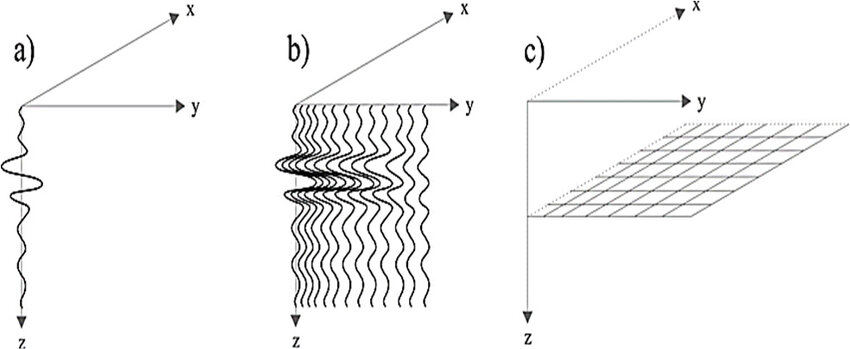
\includegraphics[scale=0.5]{gambar/scanModes.png}
  \caption{Mode visualisasi sinyal GPR: (a) A-scan, (b) B-scan, and (c) C-scan \parencite{scanModes}.}
  \label{fig:scanmodes}
\end{figure}

\subsection{A-Scan}
\label{subsec:aScan}

A-Scan merupakan mode GPR yang ditampilkan dalam satu dimensi, di mana amplitudo gelombang diplot dalam fungsi waktu. 
Pada mode ini, sinyal GPR direkam dan ditampilkan sebagai amplitudo sinyal terhadap waktu. 
Sinyal ini mencerminkan pantulan gelombang elektromagnetik yang terdeteksi oleh GPR saat menjelajahi lapisan tanah atau struktur di bawah permukaan.

Dalam mode A-scan, sumbu waktu merepresentasikan jarak atau posisi relatif dari antena GPR saat menjelajahi lapisan tanah atau struktur di bawah permukaan. 
Titik awal grafik A-scan mengindikasikan saat gelombang elektromagnetik dipancarkan oleh antena GPR, dan titik akhirnya mencerminkan waktu yang dibutuhkan untuk gelombang elektromagnetik mencapai target atau objek bawah permukaan dan kembali ke antena GPR.
Sedangkan Amplitudo sinyal pada sumbu vertikal menunjukkan kekuatan atau intensitas sinyal GPR yang terdeteksi oleh antena saat berinteraksi dengan benda atau lapisan bawah permukaan. 
Puncak amplitudo yang tinggi menunjukkan adanya pantulan kuat, sedangkan amplitudo yang lebih rendah menunjukkan adanya pantulan yang lebih lemah.

Gambar \ref{fig:AscanGPR} merupakan contoh dari grafik A-Scan pada simulasi gprMax yang ditampilkan dalam 6 jenis grafik. 
Untuk setiap barisnya merupakan grafik A-scan berdasarkan sumbu acuan (sumbu-x, sumbu-y, dan sumbu-z), sedangkan setiap kolomnya merupakan grafik A-scan berdasarkan kuat bidang elektromagnetik (kuat medan listrik (E) dan kuat medan magnet (H))
Pada grafik, terlihat grafik sinyal A-scan untuk kuat medan listrik pada sumbu-x dan sumbu-y, serta kuat medan magnet pada sumbu-z selalu bernilai 0.
Hal ini menunjukkan pada simulasi gprMax, sinyal GPR dipancarkan secara vertikal (sumbu-z) ke arah bawah suatu permukaan.

\begin{figure}[ht]
  \centering
  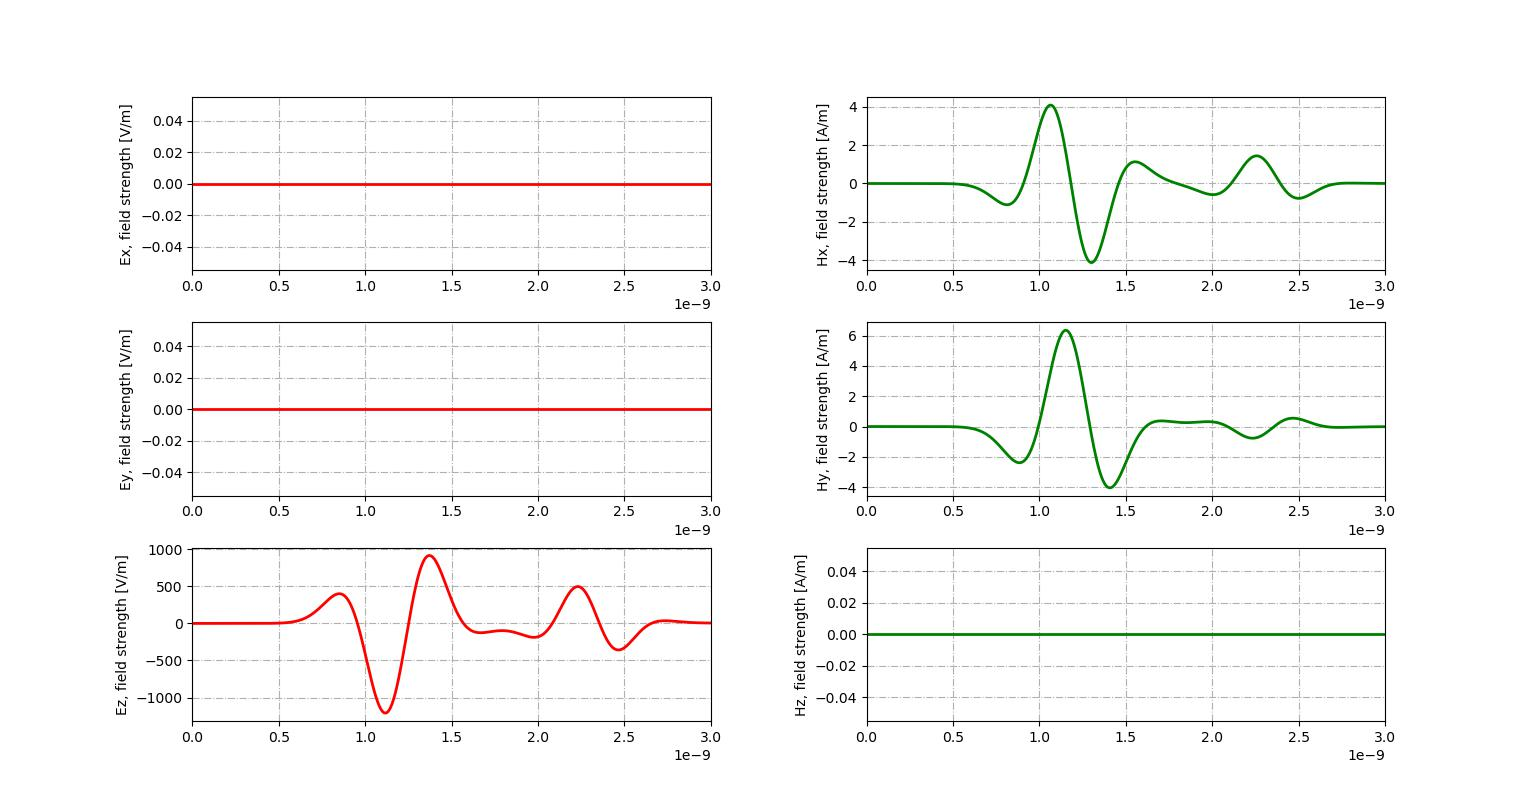
\includegraphics[scale=0.45]{gambar/GPRAscan.jpeg}
  \caption{Contoh A-Scan Sinyal GPR.}
  \label{fig:AscanGPR}
\end{figure}

Bentuk gelombang tunggal atau A-Scan didefinisikan sebagai

\begin{equation}
  \label{eq:Ascan}
  F(z)=A( x_{i} , y_{j} , z_{k} )
\end{equation}

di mana rentang k = 1 sampai N, i dan j bilangan konstan \parencite{danielDvd}.\\

\subsection{B-Scan}
\label{subsec:bScan}

B-scan merupakan sebuah set dari gelombang A-scan GPR yang berurutan sepanjang arah tertentu. 
Mode B-scan menghasilkan gambar 2 dimensi dari data GPR, yang berguna untuk memberikan gambaran keseluruhan dari struktur yang dilintasi oleh GPR.
Dengan melihat gambar B-scan, pengguna GPR dapat mengidentifikasi batas lapisan, perubahan komposisi material, atau adanya objek tertanam seperti pipa, kabel, atau struktur bawah permukaan lainnya.

Dalam mode B-scan, sumbu horizontal pada gambar menunjukkan posisi lintasan perangkat GPR saat pemindaian, sedangkan sumbu vertikal merepresentasikan kedalaman atau jarak relatif. 
Setiap titik pada gambar B-scan mewakili amplitudo atau kekuatan sinyal GPR yang terdeteksi pada posisi tersebut. 
Gambar B-scan biasanya ditampilkan dalam skala abu-abu atau dalam warna dengan gradasi intensitas yang menggambarkan kekuatan sinyal.

\begin{figure}[ht]
  \centering
  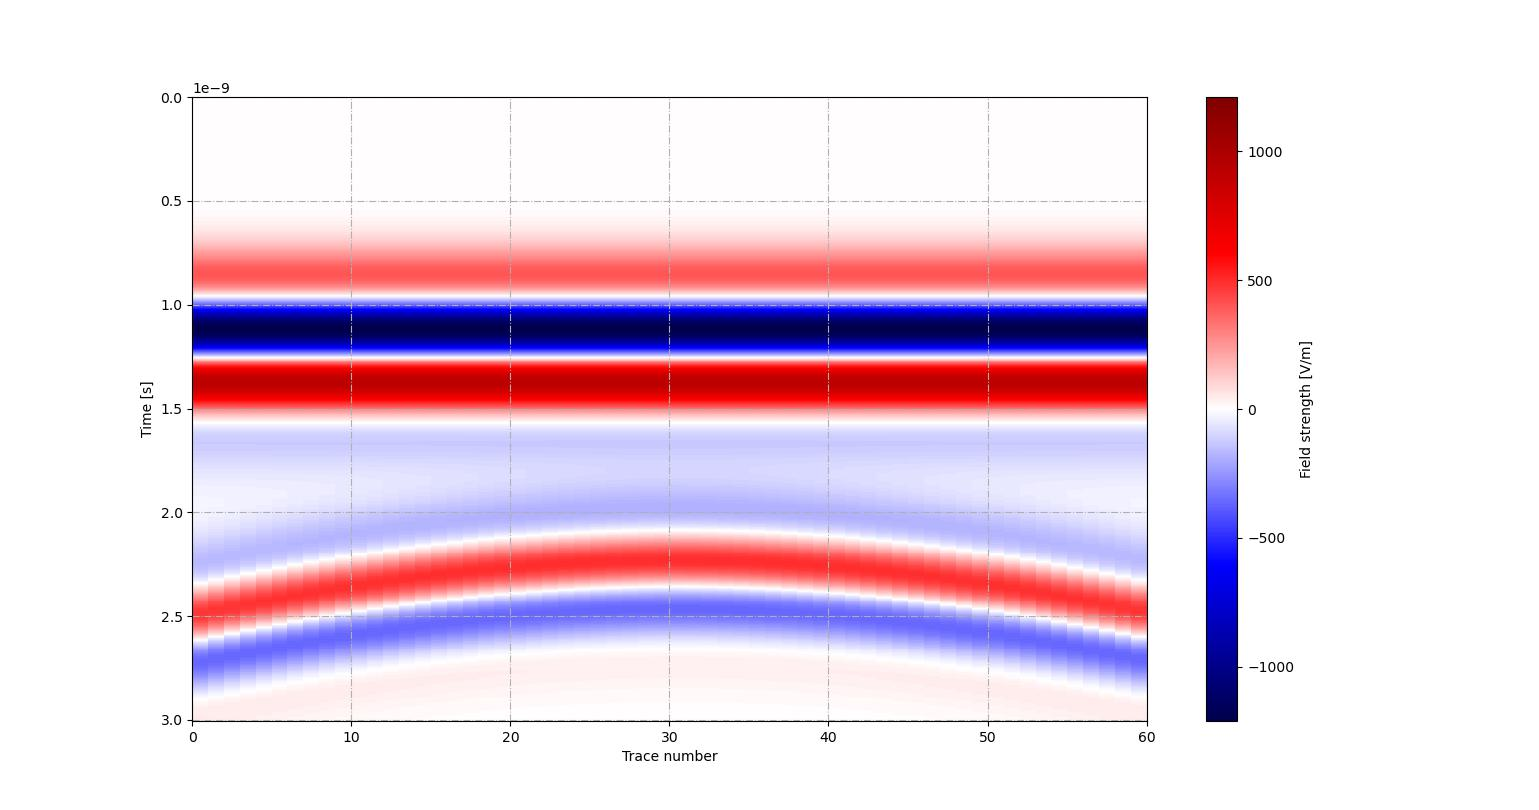
\includegraphics[scale=0.45]{gambar/GPRBscan.jpg}
  \caption{Contoh B-Scan Sinyal GPR.}
  \label{fig:BscanGPR}
\end{figure}

Gambar \ref{fig:BscanGPR} merupakan contoh dari bentuk B-Scan pada simulasi gprMax. 
Gambar B-scan ditampilkan berwarna dengan gradasi warna merah-biru. 
Pada keterangan gradasi warna gambar, warna merah menunjukkan sinyal kuat (nilai positif) dan warna biru menunjukkan sinyal lemah (nilai negatif) dengan interval nilai medan listrik (Ez) dari -1000 $V.m^{-1}$ hingga 1000 $V.m^{-1}$.

Dalam gambar B-scan, bentuk parabola sinyal muncul karena adanya perbedaan konduktivitas atau dielektrik antara lapisan atau objek yang terdeteksi. 
Ketika gelombang elektromagnetik melewati batas antara dua bahan yang berbeda, terjadi pembiasan dan perubahan arah lintasan gelombang.
Hal ini mengakibatkan adanya variasi amplitudo sinyal yang terdeteksi.

Pada gambar \ref{fig:BscanGPR}, perubahan warna merah-biru dan kebalikannya pada sinyal B-scan biasanya mewakili perubahan amplitudo atau kekuatan sinyal yang terdeteksi oleh GPR. 
Perubahan warna ini dapat disebabkan oleh beberapa faktor, yaitu : 

\begin{enumerate}[nolistsep]

  \item Perbedaan konduktivitas material.
  
  Material dengan konduktivitas yang lebih tinggi atau kemampuan untuk memantulkan gelombang elektromagnetik secara lebih baik akan menghasilkan sinyal yang lebih kuat dan warna yang lebih terang (merah) dalam gambar B-scan. 
  Sebaliknya, material dengan konduktivitas rendah atau kemampuan refleksi yang lebih rendah akan menghasilkan sinyal yang lebih lemah dan warna yang lebih gelap (biru).   

  \item Perbedaan bentuk geometri objek.
  
  Objek dengan bentuk yang mengarahkan atau memfokuskan gelombang elektromagnetik ke antena GPR dapat menghasilkan sinyal yang lebih kuat dan warna yang lebih terang (merah). 
  Sebaliknya, objek dengan geometri yang mengakibatkan penyebaran atau dispersi gelombang elektromagnetik akan menghasilkan sinyal yang lebih lemah dan warna yang lebih gelap (biru).

  \item Jarak tempuh gelombang.
  
  Semakin jauh jarak tempuh gelombang elektromagnetik, semakin lemah intensitas sinyal yang terdeteksi. 
\end{enumerate}

Bentuk gelombang dua dimensi atau B-Scan didefinisikan sebagai

\begin{equation}
  \label{eq:Bscanx}
  F(x,z)=A( x_{i} , y_{j} , z_{k} )
\end{equation}

di mana rentang k = 1 sampai N, i = 1 sampai L, dan j bilangan konstan, atau

\begin{equation}
  \label{eq:Bscany}
  F(y,z)=A( x_{i} , y_{j} , z_{k} )
\end{equation}

di mana rentang k = 1 sampai N, j = 1 sampai M, dan i bilangan konstan \parencite{danielDvd}.

\subsection{Bandwidth}
\label{subsec:bandwidth}

\emph{Bandwidth} merupakan perbedaan antara batas frekuensi tertinggi dengan frekuensi terendah sinyal. 
Pengukuran \emph{Bandwidth} berhubungan langsung dengan resolusi. 
Durasi waktu dari pulsa transmisi berbanding terbalik dengan \emph{bandwidth}. 
Secara matematis, nilai \emph{bandwidth} dan durasi waktu dapat didefinisikan sebagai berikut

\begin{equation}
  \label{eq:BW}
  B \geq  \frac{v}{4 \Delta r} 
\end{equation}

di mana r merupakan panjang resolusi dan v merupakan kecepatan perambatan \parencite{jol2008ground}.

\subsection{Center Frequency}
\label{subsec:centerFrequency}

\emph{Center frequency} merupakan titik tengah dari batas frekuensi atas dan frekuensi bawah. 
\emph{Bandwidth} tidak menentukan frekuensi dari sinyal GPR, namun dapat menentukan batas frekuensi dari \emph{center frequency}.
Semakin rendah frekuensi, semakin besar kemungkinan mendapat sinyal GPR dari media perambatnya.

Sinyal GPR dicirikan oleh rasio bandwidth terhadap \emph{center frequency}

\begin{equation}
  \label{eq:cF}
  R =  \frac{B}{ f_{c} } 
\end{equation}

di mana rasio R diusakan sebesar mungkin \parencite{jol2008ground}. 
Umumnya GPR mencapai rasio R mendekati 1, sehingga \emph{bandwidth} biasa ditafsirkan bernilai sama dengan nilai \emph{center frequency}.

\subsection{Ricker Wavelet}
\label{subsec:rickerWavelet}

Pada GPR, metode pembangkitan data Ricker Wavelet merupakan salah satu metode terbaik dalam membangkitkan data seismik \parencite{rickeronSeismic}. 
Wavelet merupakan satu gelombang pendek, yang diperoleh dari suatu model matematik. 
Wavelet Ricker memungkinkan untuk menggunakan sedikit parameter dalam mendeteksi sinyal seismik.

Ricker wavelet didefinisikan dalam domain waktu sebagai

\begin{equation}
  \label{eq:rickerTimeDomain}
  r(t) =  \big(1 -  \frac{1}{2} (  \omega _{p} ^{2}  t^{2} ) \big)  . exp \big(- \frac{1}{4} ( \omega _{p} ^{2}  t^{2} ) \big) 
\end{equation}

di mana t merupakan waktu dan $\omega_{p}$ merupakan frekuensi sudut puncak.

Spektrum frekuensi dari ricker wavelet dapat didefinisikan sebagai

\begin{equation}
  \label{eq:rickerTimeDomain}
  R( \omega ) =  \big( \frac{2 \omega ^{2}}{  \sqrt{ \pi }  \omega _{p} ^{3}} \big)  . exp \big(- \frac{ \omega ^{2}}{ \omega _{p} ^{2}} \big) 
\end{equation}

\begin{figure}[ht]
  \centering
  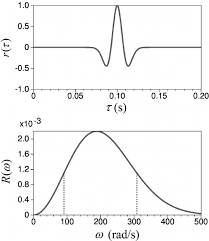
\includegraphics[scale=1]{gambar/ricker.jpg}
  \caption{Grafik gelombang ricker beserta spektrum frekuensi \parencite{rickerWavelet}.}
  \label{fig:gelombangRicker}
\end{figure}

Grafik ricker wavelet beserta spektrum frekuensi ditampilkan pada gambar \ref{fig:gelombangRicker}. 
Pada gambar tersebut, digunakan frekuensi sudut puncak $\omega$ = 60$\pi$ rad/s

\section{Neural Networks}
\label{sec:neuralNetworks}

\emph{Neural Network} merupakan salah satu bagian dari \emph{machine learning} yang terinspirasi dari bentuk jaringan neuron pada otak manusia. 
Setiap neuron atau node akan dikumpulkan dalam suatu lapisan (\emph{layers}), yang akan saling berhubungan dan berurutan. 
Pada tingkat paling dasarnya, sebuah jaringan terdiri dari satu node yang mengambil input vektor dikali bobot tertentu, kemudian diubah dengan transformasi non-linear untuk mencapai output yang diharapkan. 
Jaringan juga memiliki lapisan tersembunyi (\emph{hidden layers}), yang beratnya dapat dioptimalkan dalam mencapai output yang diharapkan.

\subsection{Deep Learning}
\label{subsesc:deeplearning}
\emph{Deep learning} merupakan algoritma yang menggunakan \emph{artificial neural networks} (ANN). 
ANN kemungkinan dianggap sebagai cara yang paling baik dalam menentukan serangkaian fungsi yang fleksibel. 
Hal ini dikarenakan ANN dibangun dari banyak blok komputasi dasar yang disebut neuron. 
Secara khusus, daripada memprogram serangkaian instruksi khusus untuk menyelesaikan masalah secara langsung, model \emph{deep learning} dilatih berdasarkan data dari dunia nyata dan mempelajari bagaimana cara menyelesaikan masalah \parencite{PDLT-2022}. 

\subsection{Convolutional Neural Network}
\label{subsec:convolutionalNeuralNetwork}

Dalam \emph{deep learning}, \emph{Convolutional Neural Network} (CNN) adalah kelas jaringan saraf tiruan yang paling umum diterapkan untuk menganalisis citra visual. 
Convolutional Neural Network (CNN) telah menunjukkan kinerja yang sangat baik dalam banyak masalah visi komputer dan \emph{machine learning}. 
Banyak paper yang telah diterbitkan tentang topik ini, dan beberapa \emph{open source software} CNN telah tersedia. 
CNN berguna dalam banyak aplikasi, terutama dalam tugas-tugas terkait gambar. 
Aplikasi CNN termasuk klasifikasi gambar, segmentasi semantik gambar, deteksi objek dalam gambar, dsb \parencite{introductionCNN}. 

\section{Model Generatif}
\label{sec:modelGeneratif}

Model generatif merupakan bagian dari \emph{Neural Network} yang memungkinkan upaya sintesis dara yang realistis. 
Dasar dari model ini terletak pada \emph{neural network} yang berfungsi secara universal. 
Model ini memungkinkan model, yang awalnya diberi input, mempelajari fitur dari input tersebut, kemudian mampu menghasilkan output yang mirip dengan data input.

\subsection{Generative Adversarial Network}
\label{subsec:generativeAdversarialNetwork}

\emph{Generative Adversarial Network} (GAN) adalah bentuk model generatif, di mana model dibagi menjadi 2 bagian, yaitu bagian generatif (G) dan bagian diskriminator (D). 
Bagian generatif merupakan bagian untuk mensintesis data, sedangkan bagian diskriminator merupakan bagian untuk menentukan apakah data sintesis merupakan data palsu atau asli. 
Model ini seringkali diaplikasikan untuk mereplikasi suatu data, seperti gambar, video, dan audio.

Generator dan Diskriminator akan saling menguntung-rugikan, dengan fungsi V(D,G) direpresentasikan sebagai berikut : 

\begin{equation}
  \label{eq:GAN}
  min_{G} max_{D} V(G,D) =  E_{x \sim p_{data} (x)} \big[ log D(x) \big] + E_{z \sim p_{z} (z)} \big[ log  \big(1-D \big(G(z)\big) \big) \big]
\end{equation}

Dalam mempelajari distribusi generator p pada data x, variabel kebisingan input pz(z) didefinisikan sebelumnya, kemudian pemetaan direpresentasikan ke ruang data sebagai G(z; (teta)g), di mana G adalah fungsi diferensiasi yang direpresentasikan oleh multilayer perceptron dengan parameter (teta)g. 
Multilayer perceptron (MLP) kedua D(x; (teta)d) yang menghasilkan skalar tunggal juga didefinisikan. 
D(x) merepresentasikan kemungkinan bahwa x berasal dari data daripada pg. 
Diskriminator dilatih untuk memaksimalkan kemungkinan menempatkan label yang benar untuk data pelatihan dan sampel dari Generator. 
Generator dan  Diskriminator dilatih secara bersamaan untuk meminimalkan log(1-D(G(z))). \parencite{GAN}

\subsection{Conditional Generative Adversarial Network}
\label{subsec:conditionalGAN}

\emph{Generative Adversarial Network} dapat diperluas ke model bersyarat jika generator dan diskriminator dikondisikan pada beberapa informasi tambahan y. 
Konstanta y bisa berupa segala jenis informasi tambahan, seperti label kelas atau data dari modalitas lain. 
Pengkondisian juga dapat dilakukan dengan memasukkan y ke dalam diskriminator dan generator sebagai lapisan masukan tambahan.

Fungsi dari untung rugi Generator dan Diskriminator V(D,G) untuk \emph{Conditional Generative Adversarial Network} (CGAN) direpresentasikan sebagai berikut :

\begin{equation}
  \label{eq:CGAN}
  min_{G} max_{D} V(G,D) =  E_{x \sim p_{data} (x)} \big[ log D(x|y) \big] + E_{z \sim p_{z} (z)} \big[ log  \big(1-D \big(G(z|y)\big) \big) \big]
\end{equation}

Dalam generator, input kebisingan sebelumnya, pz(z), dan y digabungkan dalam representasi tersembunyi gabungan, dan kerangka pelatihan adversarial memungkinkan fleksibilitas yang cukup besar dalam bagaimana representasi tersembunyi ini disusun. 
Dalam diskriminator x dan y disajikan sebagai input dan ke fungsi diskriminatif (dalam kasus ini diwujudkan kembali oleh MLP). \parencite{CGAN}

\section{Loss Function}
\label{sec:lossFunction}

\emph{Loss Function} merupakan fungsi yang membandingkan target dengan nilai output yang diprediksi. 
Fungsi ini mengukur seberapa baik suatu \emph{Neural Network} memodelkan data pelatihan. 
Saat pelatihan, model akan meminimalkan nilai \emph{Loss Function} antara output yang diprediksi dan target.

\subsection{Sigmoid Cross-Entropy Loss}
\label{sigmoidCrossEntropyLoss}

\emph{Sigmoid function} merupakan fungsi kontinu berbentuk “S” dengan range dari 0 sampai 1 untuk domain bilangan riil. 
Fungsi sigmoid adalah fungsi yang paling umum dikenal digunakan dalam \emph{Feedforward Neural Network} (FNN) karena sifat nonlinier dan kesederhanaan komputasi turunannya. 
Bentuk sederhana dari fungsi sigmoid secara matematis didefinisikan sebagai 

\begin{equation}
  \label{eq:sigmoid}
  f(h) =  \frac{1}{1+exp(-2 \beta h)} 
\end{equation}

dimana $\beta$ merupakan konstanta atau parameter yang dapat dilatih dan fungsi memenuhi kondisi f(h) + f(-h) = 1 \parencite{sigmoid}. Bentuk grafik fungsi sigmoid dapat dilihat pada gambar \ref{fig:sigmoid}

\begin{figure}[ht]
  \centering
  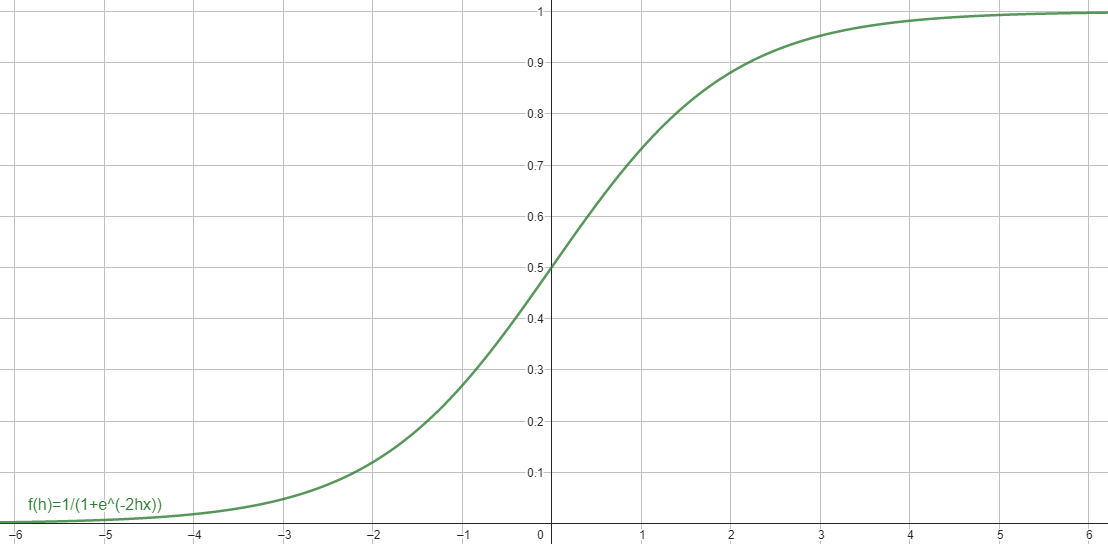
\includegraphics[scale=0.35]{gambar/sigmoid.png}
  \caption{Grafik Fungsi Sigmoid.}
  \label{fig:sigmoid}
\end{figure}

\emph{Sigmoid cross-entropy loss}, juga dikenal sebagai \emph{binary cross-entropy loss} \parencite{lossFunction}, merupakan fungsi yang digunakan untuk mengukur perbedaan antara prediksi yang dihasilkan oleh model dan label yang sebenarnya pada kasus klasifikasi biner, di mana setiap sampel data hanya dapat memiliki dua kelas yang mungkin. 
Fungsi \emph{sigmoid cross-entropy loss} menggunakan fungsi sigmoid untuk memetakan nilai prediksi yang kontinu ke dalam rentang antara 0 dan 1. 
Selanjutnya, fungsi ini membandingkan nilai prediksi yang dihasilkan dengan label yang sebenarnya menggunakan matriks \emph{loss cross-entropy}. 
Secara matematis, fungsi \emph{sigmoid cross-entropy loss} didefinisikan sebagai 

\begin{equation}
  \label{eq:sigmoidCrossEntropyLoss}
  L_{log} = H(f,y) = - \frac{1}{N}  \sum_ {i=1} ^N  \big( y_{i} . log \big(f( y_{i} ) \big) +(1 - y_{i}) . log \big(1 - f( y_{i} ) \big) \big)  
\end{equation}

dimana $y_{i}$ merupakan label untuk titik tertentu (0 untuk warna hijau dan 1 untuk warna merah) dan f(y) merupakan fungsi sigmoid untuk memprediksi probabilitas suatu titik bernilai 0 (hijau) untuk semua titik N.

\subsection{Image Differencing}
\label{imagediff}

\emph{Image differencing} merupakan metode pengurangan nilai digital dari suatu gambar dengan gambar lain. 
Metode ini akan mengurangi nilai setiap piksel gambar yang berada di posisi yang sama, kemudian hasil pengurangan akan ditampilkan dalam bentuk gambar. 
Secara matematis, metode image differencing didefinisikan sebagai

\begin{equation}
  \label{eq:imagediff}
  l_{d}(x,y) =  l_{1}(x,y) - l_{2}(x,y) 
\end{equation}

dimana $l_{1}$ dan $l_{2}$ merupakan kedua gambar input dan (x,y) merupakan posisi pixel \parencite{imgdiff}.

\subsection{Mean Squared Error}
\label{subsec:MSE}

\emph{Mean Squared Error} (MSE) adalah rata-rata error kuadrat antara nilai aktual dan prediksi. 
Dalam model yang memprediksi variabel kontinu, MSE adalah tolok ukur kinerja yang ideal karena keterkaitannya dengan konsep \emph{cross-entropy} dari teori informasi. 
\emph{Cross-entropy} akan mengukur kesamaan dua distribusi probabilitas. 
Jika tujuan pemodelan adalah untuk mengidentifikasi model yang paling dekat mereproduksi distribusi penghasil data yang sebenarnya, maka model terbaik akan meminimalkan \emph{cross-entropy} antara prediksi model dan data pelatihan \parencite{MSE}. 

\subsection{Structural Similarity Index Measurement}
\label{subsec:SSIM}

\emph{Structural Similarity Index Measurement} (SSIM) adalah metode yang digunakan untuk mengukur kesamaan struktural antara dua gambar atau sinyal. 
Metrik ini dikembangkan untuk mencerminkan persepsi visual manusia dalam mengevaluasi kesamaan antara dua gambar. 
SSIM memperhitungkan 3 parameter yang ada pada citra, yaitu kecerahan (\emph{luminance}), kontras (\emph{contrast}), dan struktur (\emph{structure}). 
Diagram sistem SSIM dapat dilihat pada gambar berikut.

\begin{figure}[ht]
  \centering
  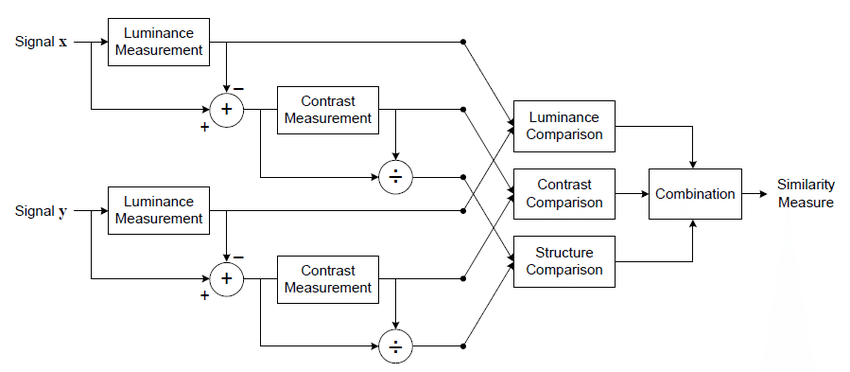
\includegraphics[scale=0.5]{gambar/SSIM.png}
  \caption{Diagram Sistem SSIM \parencite{SSIM}.}
  \label{fig:SSIM}
\end{figure}

Secara matematis, nilai SSIM dari 2 gambar (x, y) didefinisikan sebagai 

\begin{equation}
  \label{eq:ssim1}
  SSIM(x,y) =  [l(x,y)^{ \alpha } ] . [c(x,y)^{ \beta }].[s(x,y)^{ \gamma }]
\end{equation}

dimana $\alpha$, $\beta$ dan $\gamma$ bilangan positif yang merupakan parameter yang digunakan untuk menyesuaikan tingkat kepentingan relatif dari ketiga komponen tersebut. 
Dengan mengasumsikan ketiga komponen memiliki tingkat kepentingan yang sama ($\alpha$=$\beta$=$\gamma$=1), maka nilai SSIM secara spesifik didefinisikan sebagai 

\begin{equation}
  \label{eq:ssim2}
  SSIM(x,y) =  \frac{(2  \mu_{x} \mu_{y} + C_{1})(2 \sigma_{xy} + C_{2} )}{(\mu_{x}^{2}  + \mu_{y}^{2}+C_{1})(\sigma_{x}^{2}+\sigma_{y}^{2}+C_{2})} 
\end{equation}

dimana $\mu$ merupakan nilai rata-rata dari intensitas piksel, $\sigma$ merupakan estimasi dari kontras gambar, dan C1 C2 merupakan konstanta untuk menghindari ketidakstabilan \parencite{SSIM}.

\section{Adam Optimizer}
\label{adamOptimizer}

Adam merupakan sebuah metode untuk optimasi stokastik yang efisien, yang hanya membutuhkan gradien orde pertama dengan sedikit kebutuhan memori. 
Nama Adam diambil dari singkatan \emph{adaptive moment estimation}. 
Metode ini mudah diimplementasikan, efisien secara komputasi, memiliki sedikit kebutuhan memori, tidak berubah terhadap penskalaan diagonal gradien, dan cocok untuk masalah yang besar dalam hal data dan/atau parameter. 
Metode ini merupakan gabungan dari dua metode, yaitu AdaGrad \parencite{adaGrad}, yang bekerja dengan baik dengan gradien sparse, 
dan RMSProp \parencite{RMSProp}, yang bekerja dengan baik di pengaturan \emph{on-line} dan \emph{non-stationary}\parencite{adam}.